% intro.tex

%%%%%%%%%%%%%%%%%%%%
\begin{frame}{Transaction and Isolation Level}
  \begin{center}
    A transaction is a \blue{\it group} of operations
    that is executed \red{atomically}.

    \vspace{0.30cm}
		\resizebox{0.60\textwidth}{!}{% isolation-intro-write-skew-tikz.tex

\begin{tikzpicture}[
  node distance = 1.5cm and 1.5cm,
  txn/.style = {draw, inner sep = 3pt, align = left},
  comm/.style = {arrows = {Stealth-Stealth}, ultra thick, purple}]

  \uncover<2->{
  \node[txn] (t-alice)
    {$x_{1} \gets \readevent(\acctone)$\\[2pt]
     $x_{2} \gets \readevent(\accttwo)$\\[2pt]
     $\text{\bf if}\; x_{1} + x_{2} > 100$ \\[2pt]
     $\quad \red{x_{1} \gets x_{1} - 100}$ \\[2pt]
     $\quad \writeevent(\acctone, x_{1})$};
  }

  \node[txn, right = of t-alice] (t-bob)
    {$x_{1} \gets \readevent(\acctone)$\\[2pt]
     $x_{2} \gets \readevent(\accttwo)$\\[2pt]
     $\text{\bf if}\; x_{1} + x_{2} > 100$ \\[2pt]
     $\quad \red{x_{2} \gets x_{2} - 100}$ \\[2pt]
     $\quad \writeevent(\accttwo, x_{2})$};

  \uncover<2->{
  \node[txn, right = of t-bob] (t-carol)
    {$x_{1} \gets \readevent(\acctone)$\\[2pt]
     $x_{2} \gets \readevent(\accttwo)$};
  }

  \uncover<3->{
  \node[draw, fill = yellow!50, below = of t-bob, font = \large,
    inner sep = 8pt] (isolation)
    {{Isolation Level (aka Transactional Consistency Model)}};
  }

  \node[below = of isolation,
    label = {[label distance = 5pt]above : {\large $\acctone = \accttwo = 60$}}] (db)
    {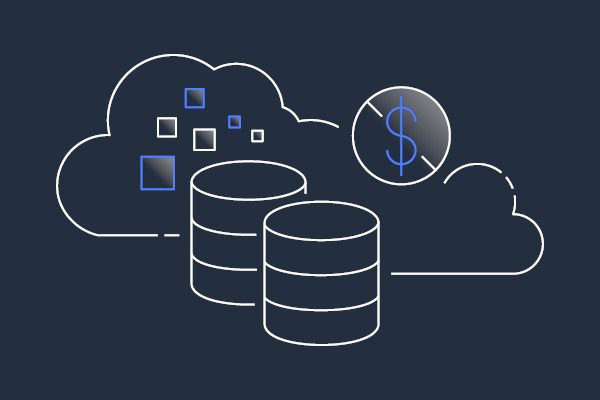
\includegraphics[scale = 0.75]{figs/db-logo-dollar}};

  \uncover<1>{
  \draw[comm] (t-bob) -- (db);
  }

  \uncover<3->{
  \draw[comm] (t-alice) -- (t-alice |- isolation.north);
  \draw[comm] (t-bob) -- (t-bob |- isolation.north);
  \draw[comm] (t-carol) -- (t-carol |- isolation.north);
  \draw[comm] (isolation) -- (isolation |- db.north);
  }
\end{tikzpicture}}

    \vspace{0.20cm}
    \uncover<3->{
      The isolation levels specify how they are isolated from each other.
    }
  \end{center}
\end{frame}
%%%%%%%%%%%%%%%%%%%%

%%%%%%%%%%%%%%%%%%%%
\begin{frame}{Serializability (SER)}
  \begin{center}
    All transactions appear to execute in some total order.

    \vspace{0.30cm}
		\resizebox{0.50\textwidth}{!}{% isolation-ser-write-skew-tikz.tex

\begin{tikzpicture}[
  node distance = 1.5cm and 1.5cm,
  txn/.style = {draw, inner sep = 3pt, align = center},
  comm/.style = {arrows = {Stealth-Stealth}, ultra thick, purple}]

  \node[txn] (t-alice)
    {$x_{1} \gets \readevent(\acctone)$\\[2pt]
     $x_{2} \gets \readevent(\accttwo)$\\[2pt]
     $\text{\bf if}\; x_{1} + x_{2} > 100$ \\[2pt]
     $\quad \red{x_{1} \gets x_{1} - 100}$ \\[2pt]
     $\quad \writeevent(\acctone, x_{1})$};

  \node[txn, right = of t-alice] (t-bob)
    {$x_{1} \gets \readevent(\acctone)$\\[2pt]
     $x_{2} \gets \readevent(\accttwo)$\\[2pt]
     $\text{\bf if}\; x_{1} + x_{2} > 100$ \\[2pt]
     $\quad \red{x_{2} \gets x_{2} - 100}$ \\[2pt]
     $\quad \writeevent(\accttwo, x_{2})$};

  \node[txn, right = of t-bob] (t-carol)
    {$x_{1} \gets \readevent(\acctone)$\\[2pt]
     $x_{2} \gets \readevent(\accttwo)$};

  \node[draw, fill = yellow!50, below = of t-bob, font = \large,
    inner sep = 8pt, minimum width = 260pt] (isolation)
    {{Serializability (SER)}};

  \node[below = of isolation,
    label = {[label distance = 5pt]above : {\large $\acctone = \accttwo = 60$}}] (db)
    {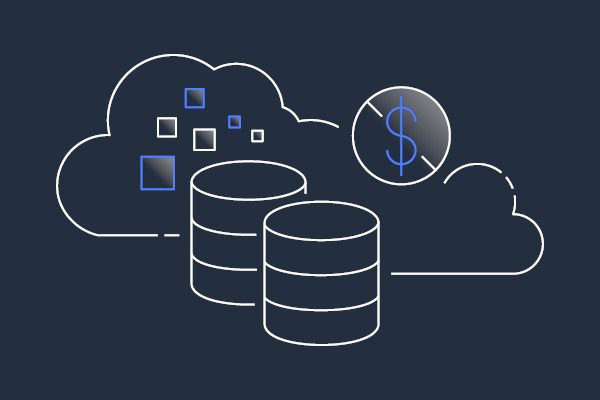
\includegraphics[scale = 0.70]{figs/db-logo-dollar}};

  \draw[comm] (t-alice) -- (t-alice |- isolation.north);
  \draw[comm] (t-bob) -- (t-bob |- isolation.north);
  \draw[comm] (t-carol) -- (t-carol |- isolation.north);
  \draw[comm] (isolation) -- (isolation |- db.north);

  \uncover<3->{
  \node[txn, below = 0.50cm of db, fill = green!30] (t-bob-execution)
    {$\readevent(\acctone, 60)$ \\[2pt]
     $\readevent(\accttwo, 60)$};
  }

  \uncover<2->{
  \node[txn, left = of t-bob-execution] (t-alice-execution)
    {$\readevent(\acctone, 60)$ \\[2pt]
     $\readevent(\accttwo, 60)$ \\[2pt]
     $\writeevent(\acctone, -40)$};
  }

  \uncover<4->{
  \node[txn, right = of t-bob-execution] (t-carol-execution)
    {$\readevent(\acctone, 60)$ \\[2pt]
     $\readevent(\accttwo, 60)$};
  }
\end{tikzpicture}}

    \vspace{0.20cm}
    \uncover<5->{
      too expensive, especially for distributed transactions
    }
  \end{center}
\end{frame}
%%%%%%%%%%%%%%%%%%%%

%%%%%%%%%%%%%%%%%%%%
\begin{frame}{Snapshot Isolation (SI)}
  \begin{center}
		\resizebox{0.50\textwidth}{!}{% isolation-si-write-skew-tikz.tex

\begin{tikzpicture}[
  node distance = 1.5cm and 1.5cm,
  txn/.style = {draw, inner sep = 3pt, align = center},
  comm/.style = {arrows = {Stealth-Stealth}, ultra thick, purple}]

  \node[txn] (t-alice)
    {$x_{1} \gets \readevent(\acctone)$\\[2pt]
     $x_{2} \gets \readevent(\accttwo)$\\[2pt]
     $\text{\bf if}\; x_{1} + x_{2} > 100$ \\[2pt]
     $\quad \red{x_{1} \gets x_{1} - 100}$ \\[2pt]
     $\quad \writeevent(\acctone, x_{1})$};

  \node[txn, right = of t-alice] (t-bob)
    {$x_{1} \gets \readevent(\acctone)$\\[2pt]
     $x_{2} \gets \readevent(\accttwo)$\\[2pt]
     $\text{\bf if}\; x_{1} + x_{2} > 100$ \\[2pt]
     $\quad \red{x_{2} \gets x_{2} - 100}$ \\[2pt]
     $\quad \writeevent(\accttwo, x_{2})$};

  \node[txn, right = of t-bob] (t-carol)
    {$x_{1} \gets \readevent(\acctone)$\\[2pt]
     $x_{2} \gets \readevent(\accttwo)$};

  \node[draw, fill = yellow!50, below = of t-bob, font = \large,
    inner sep = 8pt, minimum width = 260pt] (isolation)
    {{Snapshot Isolation (SI)}};

  \node[below = of isolation,
    label = {[label distance = 5pt]above : {\large $\acctone = \accttwo = 60$}}] (db)
    {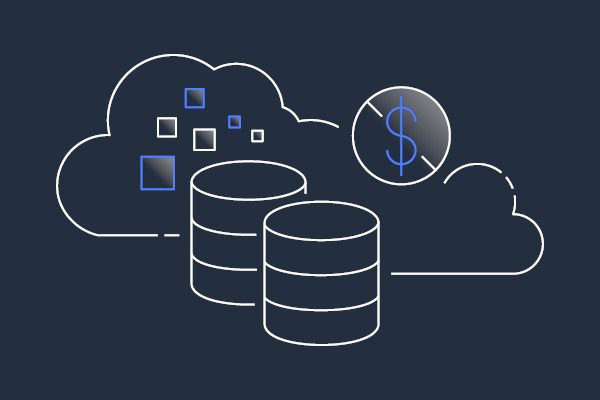
\includegraphics[scale = 0.70]{figs/db-logo-dollar}};

  \draw[comm] (t-alice) -- (t-alice |- isolation.north);
  \draw[comm] (t-bob) -- (t-bob |- isolation.north);
  \draw[comm] (t-carol) -- (t-carol |- isolation.north);
  \draw[comm] (isolation) -- (isolation |- db.north);

  \uncover<2->{
  \node[txn, below = 0.50cm of db, fill = green!30] (t-bob-execution)
    {$\readevent(\acctone, 60)$ \\[2pt]
     $\readevent(\accttwo, 60)$ \\[2pt]
     $\writeevent(\accttwo, -40)$};
  }
  \uncover<2->{
  \node[txn, left = of t-bob-execution] (t-alice-execution)
    {$\readevent(\acctone, 60)$ \\[2pt]
     $\readevent(\accttwo, 60)$ \\[2pt]
     $\writeevent(\acctone, -40)$};
  }
  \uncover<3->{
  \node[txn, right = of t-bob-execution, fill = red!30] (t-carol-execution)
    {$\readevent(\acctone, -40)$ \\[2pt]
     $\readevent(\accttwo, -40)$};

    \node[above = 1.50cm of t-carol-execution] (write-skew)
      {\green{\Large \textsc{Write Skew}}};
    \node[above = 0.80cm of t-carol-execution, scale = 3] (yes) {\yes};
  }
\end{tikzpicture}}

    \vspace{0.20cm}
    \uncover<7->{
      \violet{Snapshot Read:} Each transaction reads data from a {\it snapshot}
        of committed data valid as of the (logical) time the transaction started.
    }
  \end{center}
\end{frame}
%%%%%%%%%%%%%%%%%%%%

%%%%%%%%%%%%%%%%%%%%
\begin{frame}{Snapshot Isolation (SI)}
  \begin{center}
    \resizebox{0.48\textwidth}{!}{% isolation-si-lost-update-tikz.tex

\begin{tikzpicture}[
  node distance = 1.5cm and 1.5cm,
  txn/.style = {draw, inner sep = 3pt, align = center},
  comm/.style = {arrows = {Stealth-Stealth}, ultra thick, purple}]

  \node[txn] (t-alice)
    {$x \gets \readevent(\acct)$ \\[2pt]
     $x \gets x + 50$ \\[2pt]
     $\writeevent(\acct, x)$};

  \node[txn, right = of t-alice] (t-bob)
    {$x \gets \readevent(\acct)$ \\[2pt]
     $x \gets x + 25$ \\[2pt]
     $\writeevent(\acct, x)$};

  \node[txn, right = of t-bob] (t-carol)
    {$\readevent(\acct)$};

  \node[draw, fill = yellow!50, below = of t-bob, font = \large,
    inner sep = 8pt, minimum width = 260pt] (isolation)
    {{Snapshot Isolation (SI)}};

  \node[below = of isolation,
    label = {[label distance = 5pt]above : {\large $\acct = 0$}}] (db)
    {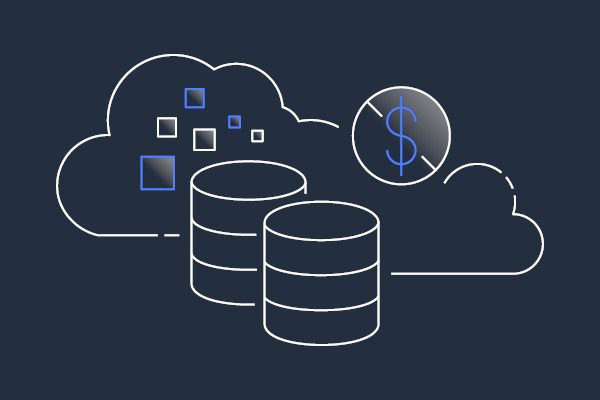
\includegraphics[scale = 0.70]{figs/db-logo-dollar}};

  \draw[comm] (t-alice) -- (t-alice |- isolation.north);
  \draw[comm] (t-bob) -- (t-bob |- isolation.north);
  \draw[comm] (t-carol) -- (t-carol |- isolation.north);
  \draw[comm] (isolation) -- (isolation |- db.north);

  \uncover<2->{
  \node[txn, below = 0.50cm of db] (t-bob-execution)
    {$\readevent(\acct, 0)$ \\[2pt] $\writeevent(\acct, ?)$};
  \node[below = 0.50cm of db, scale = 3.00] (t-bob-abort) {\no};
  }
  % \uncover<6->{
  % \node[txn, below = 0.50cm of db, fill = green!50] (t-bob-retry)
  %   {$\readevent(\acct, 0)$ \\[2pt] $\writeevent(\acct, 75)$};
  % }

  \uncover<2->{
  \node[txn, left = of t-bob-execution] (t-alice-execution)
    {$\readevent(\acct, 0)$ \\[2pt] $\writeevent(\acct, 50)$};
  }

  \uncover<2->{
  \node[above right = 0.20cm and 1.00cm of t-bob-execution] (lost-update)
    {\red{\large \textsc{Lost Update}}};
  \node[above right = -0.60cm and 1.30cm of t-bob-execution, scale = 3] (no) {\no};
  }
\end{tikzpicture}}
  \end{center}

  \vspace{-0.50cm}
  \uncover<4->{
  \violet{Snapshot Write:}
    Concurrent transactions cannot write to the same key.
    One of them must be aborted.
  }
\end{frame}
%%%%%%%%%%%%%%%%%%%%

%%%%%%%%%%%%%%%%%%%%
% \begin{frame}{Snapshot Isolation (SI)}
%   \begin{center}
%     \resizebox{0.60\textwidth}{!}{% isolation-si-causality-violation-tikz.tex

\begin{tikzpicture}[
  node distance = 1.5cm and 1.5cm,
  txn/.style = {draw, inner sep = 3pt, align = center},
  comm/.style = {arrows = {Stealth-Stealth}, ultra thick, purple}]

  \node[] (t-bob) {
\includegraphics[scale = 0.08]{figs/social-network-logo}};

  \node[draw, fill = yellow!50, below = of t-bob, font = \large,
    inner sep = 8pt, minimum width = 260pt] (isolation)
    {{Snapshot Isolation (SI)}};

  \node[below = of isolation] (db)
    {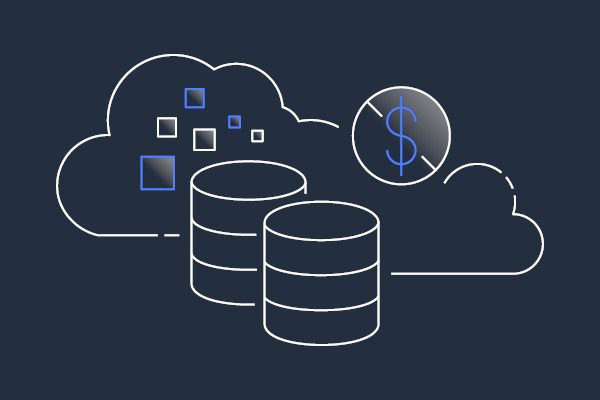
\includegraphics[scale = 0.70]{figs/db-logo-dollar}};

  \draw[comm] (t-bob) -- (t-bob |- isolation.north);
  \draw[comm] (isolation) -- (isolation |- db.north);

  \uncover<3->{
  \node[txn, below = 0.50cm of db] (t-bob-execution)
    {$\readevent(\keyxvar, \post)$ \\[2pt] $\writeevent(\keyyvar, \comment)$};
  }

  \uncover<2->{
  \node[txn, left = of t-bob-execution] (t-alice-execution)
    {$\writeevent(\keyxvar, \post)$};
  }

  \uncover<4->{
  \node[txn, right = of t-bob-execution, fill = red!30] (t-carol-execution)
    {$\readevent(\keyxvar, \emptypost)$ \\[2pt] $\readevent(\keyyvar, \comment)$};
  }
  \uncover<6->{
  \node[right = 0.10cm of t-carol-execution, scale = 2] (no-carol) {\no};
  }

  \uncover<5->{
  \node[above = of t-carol-execution] (causality-violation)
    {\red{\large \textsc{Causality Violation}}};
  }
  \uncover<6->{
  \node[above = 0.60cm of t-carol-execution, scale = 3] (no) {\no};
  }
\end{tikzpicture}}
%   \end{center}
% \end{frame}
%%%%%%%%%%%%%%%%%%%%

%%%%%%%%%%%%%%%%%%%%
\begin{frame}{Database systems and Snapshot Isolation}
  \begin{center}
    Many database systems choose to support SI.

    \vspace{0.30cm}
    \fig{width = 0.80\textwidth}{figs/db-si}
  \end{center}
\end{frame}
%%%%%%%%%%%%%%%%%%%%

%%%%%%%%%%%%%%%%%%%%
\begin{frame}{Database Systems and Snapshot Isolation}
  \begin{center}
    Database systems may \red{fail} to provide SI correctly as they claim.

    \vspace{0.30cm}
    \fig{width = 0.85\textwidth}{figs/db-si-violations}
  \end{center}
\end{frame}
%%%%%%%%%%%%%%%%%%%%

%%%%%%%%%%%%%%%%%%%%
\begin{frame}{The SI Checking Problem}
  \begin{definition}[The SI Checking Problem]
    The SI checking problem is the \purple{decision problem} of determing \\[5pt]
    whether a \teal{{\it history} $\H = (T, \SO)$} of a database system satisfies SI?
  \end{definition}

  \fig{width = 0.60\textwidth}{figs/si-checking}

  \vspace{-0.50cm}
  \[
    \SO: \text{{\it session order} among the set $T$ of transactions}
  \]
\end{frame}
%%%%%%%%%%%%%%%%%%%%

%%%%%%%%%%%%%%%%%%%%
\begin{frame}{The SI Checking Problem}
  \begin{center}
    \blue{\it Black-box SI checking:} does not rely on database internals

    \vspace{0.20cm}
    \resizebox{0.55\textwidth}{!}{% blackbox-tikz.tex

\begin{tikzpicture}[
  node distance = 1.0cm and 1.0cm,
  txn/.style = {draw, inner sep = 3pt, align = center},
  comm/.style = {arrows = {Stealth-Stealth}, ultra thick, purple}]

  \node[] (client) {
\includegraphics[scale = 0.08]{figs/client-logo}};
  \node[below = of client] (db) {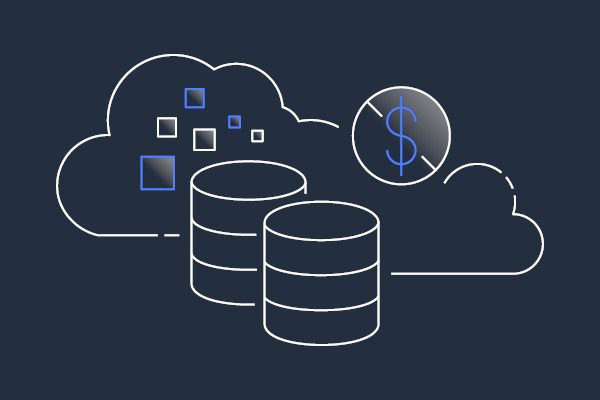
\includegraphics[scale = 0.80]{figs/db-logo-dollar}};
  \draw[comm] (client) to (db);

  \pause
  \node[txn, below = 1.00cm of db] (t-bob-execution)
    {$\readevent(\keyxvar, \post)$ \\[2pt] $\writeevent(\keyyvar, \comment)$};
  \node[txn, left = of t-bob-execution] (t-alice-execution)
    {$\writeevent(\keyxvar, \post)$};
  \node[txn, right = of t-bob-execution] (t-carol-execution)
    {$\readevent(\keyxvar, \emptypost)$ \\[2pt] $\readevent(\keyyvar, \comment)$};

  \node[draw, dashed, rectangle, inner sep = 8pt, thick,
    fit = (t-alice-execution) (t-bob-execution) (t-carol-execution)] (post) {};
  \node[right = 0.10cm of post] (lost-update)
    {\red{\large \textsc{Lost Update}}};
  \node[scale = 2] (no) at (lost-update.center) {\no};

  \pause
  \node[txn, below = 1.50cm of t-bob-execution] (t-bob-execution)
    {$\readevent(\acctone, 60)$ \\[2pt]
     $\readevent(\accttwo, 60)$ \\[2pt]
     $\writeevent(\accttwo, -40)$};
  \node[txn, left = of t-bob-execution] (t-alice-execution)
    {$\readevent(\acctone, 60)$ \\[2pt]
     $\readevent(\accttwo, 60)$ \\[2pt]
     $\writeevent(\acctone, -40)$};
  \node[txn, right = of t-bob-execution] (t-carol-execution)
    {$\readevent(\acctone, -40)$ \\[2pt]
     $\readevent(\accttwo, -40)$};
  \node[draw, dashed, rectangle, inner sep = 8pt, thick,
    fit = (t-alice-execution) (t-bob-execution) (t-carol-execution)] (acct) {};
  \node[right = 0.20cm of acct] (write-skew)
    {\red{\large \textsc{Write Skew}}};
  \node[scale = 2] (yes) at (write-skew.center) {\yes};
\end{tikzpicture}}
    \vspace{0.20cm}

    \uncover<1->{
      The histories are collected from database logs.
    }
  \end{center}
\end{frame}
%%%%%%%%%%%%%%%%%%%%

%%%%%%%%%%%%%%%%%%%%
\begin{frame}{The SI Checking Problem}
  \begin{center}
    % checker-tikz.tex

\begin{tikzpicture}[
  node distance = 0.5cm and 1.0cm,
  every label/.style = {font = \normalsize}]

	\node[draw, thick, inner sep = 8pt] (checker) {SI Checker};

	\coordinate (anchor) at ($(checker.west) + (-2.5, 0)$);
	\draw[->, thick] (anchor) to
	  node[above]{A history}
	  node[below]{$\H = (\T, \SO)$}
		(checker);

	\node[above right = of checker] (sat) {\yes};
	\node[below right = of checker] (unsat) {\no};

	\draw[->, thick] (checker) to (sat);
	\draw[->, thick] (checker) to (unsat);

	\uncover<1->{
		\node[above = 0.30cm of checker, blue] (sound) {\it Sound};
	}
	\uncover<2->{
		\node[below = 0.30cm of checker, blue] (complete) {\it Complete};
	}
	\uncover<3->{
		\node[right = 0.30cm of checker, blue] (efficient) {\it Efficient};
	}
	\uncover<4->{
		\node[below = 0.00cm of unsat, blue] (informative) {\it Informative};
	}
\end{tikzpicture}

    \vspace{0.30cm}
    \only<2>{
      \blue{\it Sound:} If the checker says \no,
        then the history does {\it not} satisfy SI.
    }
    \only<3>{
      \blue{\it Complete:} If the checker says \yes,
        then the history {\it satisfies} SI.
    }
    \only<4>{
      \blue{\it Efficient:} The checker should {\it scale} up to large workloads.
    }
    \only<5>{
      \blue{\it Informative:} The checker should provide
        understandable {\it counterexamples} if it says \no.
    }
  \end{center}
\end{frame}
%%%%%%%%%%%%%%%%%%%%

%%%%%%%%%%%%%%%%%%%%
\begin{frame}{Related Work}
  \begin{description}
    \setlength{\itemsep}{15pt}
    \item[dbcop~\ncite{Complexity:OOPSLA2019}] checker for SI \\[2pt]
      not practically efficient; \\[2pt]
      not informative, returning only ``\textsf{False}'' upon violations
    \pause
    \item[Elle~\ncite{Elle:VLDB2020}] checker for various isolation levels \\[2pt]
      \pause
      SI checking based on the Adya-style notions~\ncite{Adya:PhDThesis1999}
      relies on the start/commit timestamps of transactions.\\[2pt]
      \pause
      SI checking based on the ~\ncite{AnalysingSI:JACM2018}
      is unsound for efficiency reasons.~\footnote{https://github.com/jepsen-io/elle/issues/17; Fixed now.}
    \pause
    \item[Cobra~\ncite{Cobra:OSDI2020}] state-of-the-art checker for SER \\[2pt]
      SI checking is {\it harder} than SER checking.
  \end{description}
\end{frame}
%%%%%%%%%%%%%%%%%%%%

%%%%%%%%%%%%%%%%%%%%
\begin{frame}{Contribution: the \polysi{} Checker}
  \fig{width = 0.70\textwidth}{figs/checker-polysi}
\end{frame}
%%%%%%%%%%%%%%%%%%%%

%%%%%%%%%%%%%%%%%%%%
\begin{frame}{Contribution: the \polysi{} Checker}
  \begin{center}
    % polysi-checker-tikz.tex

\begin{tikzpicture}[
  node distance = 0.5cm and 1.0cm,
  every label/.style = {font = \normalsize}]

	\node[draw, thick, inner sep = 8pt, fill = yellow!50] (polysi) {\textsc{PolySI}};

	\coordinate (anchor) at ($(polysi.west) + (-2.5, 0)$);
	\draw[->, thick] (anchor) to
	  node[above]{A history}
	  node[below]{$\H = (\T, \SO)$}
		(polysi);

	\node[above right = of polysi] (sat) {\yes};
	\node[below right = of polysi] (unsat) {\no};

	\draw[->, thick] (polysi) to (sat);
	\draw[->, thick] (polysi) to (unsat);

	\uncover<2->{
		\node[draw, below right = 1.50cm and 0.30cm of polysi.south, fill = brown!50, inner sep = 5pt, align = center]
			(monosat) {MonoSAT \\ Solving};
	}
	\uncover<1->{
		\node[draw, below left = 1.50cm and 0.30cm of polysi.south, fill = brown!50, inner sep = 5pt, align = center]
			(encoding) {SAT \\ Encoding};
	}
	\uncover<3->{
		\node[draw, left = 0.60cm of encoding, fill = brown!50, inner sep = 5pt, align = center]
			(pruning) {Constraints \\ Pruning};
	}
	\uncover<4->{
		\node[draw, right = 0.60cm of monosat, fill = brown!50, inner sep = 5pt, align = center]
			(counterexamples) {Counterexamples \\ Extracting};
	}
	\uncover<3->{
		\draw[->, thick, brown] (pruning) to (encoding);
	}
	\uncover<2->{
		\draw[->, thick, brown] (encoding) to (monosat);
	}
	\uncover<4->{
		\draw[->, thick, brown] (monosat) to (unsat);
		\draw[->, thick, brown] (unsat) to (counterexamples);
	}

	\uncover<1->{
		\draw[dashed, very thick, blue] (polysi.south west) to (pruning.north west);
		\draw[dashed, very thick, blue] (polysi.south east) to (counterexamples.north east);
	}
\end{tikzpicture}

    \vspace{0.50cm}
    \only<2>{
      \blue{{\it Sound} \&{\it Complete:}}
        polygraph based characterization of SI
    }
    \only<3>{
      \blue{\it Efficient:} utilizing MonoSAT solver optimized for graph problems
    }
    \only<4>{
      \blue{\it Efficient:} domain-specific pruning before encoding
    }
    \only<5>{
      \blue{\it Informative:} extract counterexamples from the unsatisifiable core
    }
  \end{center}
\end{frame}
%%%%%%%%%%%%%%%%%%%%